\pdfminorversion=7
\documentclass[
  10pt,
  hyperref={
    pdfauthor={William C. Dawn},
    pdftitle={PhD QE2 Review and Critique},
    pdfcreator={pdflatex},
    pdfsubject={NCSU Nuclear Engineering PhD Qualifying Exam Part 2},
    pdfkeywords={Jacobi-free Newton-Krylov, nodal expansion method, physics-based
      preconditioner, nuclear reactor analysis},
  }
]{beamer}
%\documentclass[handout,12pt]{beamer} % includes notes
\usetheme{NCSU}

% fix conflict between beamer and subfig
\makeatletter
\let\@@magyar@captionfix\relax
\makeatother

% set font Times New Roman
\usepackage[T1]{fontenc}
\usepackage[utf8]{inputenc}
\usepackage{newtxtext,newtxmath}
\usepackage{microtype}
\usepackage{amsmath,amsfonts,amssymb}

\setbeamerfont{itemize/enumerate subbody}{size=\normalsize}
\setbeamerfont{itemize/enumerate subsubbody}{size=\small}

\usepackage[american]{babel}
\usepackage{csquotes}
\usepackage[
			style=alphabetic,%numeric-comp,%authoryear-comp,%
			sorting=nyt,%ynt					
			hyperref=true, %	
			giveninits=true,%
			backend=biber,
      bibencoding=utf8,
			natbib=true,
			url=false,
			isbn=false,
			maxnames=2, %for et al to be used
			maxalphanames=1, %to avoid printing a + for every et al in abbreviation
			doi=false,
]{biblatex}		
\addbibresource{../WilliamDawn-QE2.bib}
\renewcommand*{\labelalphaothers}{}
\renewcommand*{\bibfont}{\scriptsize}
\setbeamertemplate{bibliography item}{\insertbiblabel}

\usepackage{booktabs}

\usepackage{graphicx}

% demand a table of contents for each current section
\AtBeginSection[]
{
  \begin{frame}
    \frametitle{Outline}
    \tableofcontents[currentsection]
  \end{frame}
}

\usepackage[acronym]{glossaries}
\usepackage{acronym}
\setacronymstyle{long-short}
\makeglossaries

\newacronym{jfnk}{JFNK}{Jacobi-Free Newton-Krylov}
\newacronym{nem} {NEM} {Nodal Expansion Method}
\newacronym{casl}{CASL}{Consortium for Advanced Simulation of LWRs}

\glstocfalse
\renewcommand{\glossarysection}[2][]{}

\usepackage{xspace}

% linear algebra
\renewcommand{\epsilon}{\varepsilon} % use the pretty epsilon

% variable definitions
\newcommand{\keff}{\ensuremath{k_{\!\mbox{\scriptsize \em eff}}}\xspace}

% general macros
\newcommand{\units}[1]{\ensuremath{\left[\text{{#1}}\right]}}
\newcommand{\half}{\frac{1}{2}}

% reference macros
\newcommand{\eref}[1]{\hyperref[#1]{Eq.~}(\ref{#1})}
\newcommand{\fref}[1]{\hyperref[#1]{Fig.~}\ref{#1}}
\newcommand{\tref}[1]{\hyperref[#1]{Table~}\ref{#1}}
\newcommand{\sref}[1]{\hyperref[#1]{\S}\ref{#1}}
\newcommand{\chref}[1]{\hyperref[#1]{Chapter~}\ref{#1}}
\newcommand{\apref}[1]{\hyperref[#1]{Appendix~}\ref{#1}}
\newcommand{\algorithmref}[1]{\hyperref[#1]{Algorithm~}\ref{#1}}


% Information to be included in the title page:
\title[Ph.D. Qualifying Exam Part 2]
  {A Review and Critique of \texorpdfstring{\citetitle{qe2paper}}{Jacobian-Free 
    Newton-Krylov Nodal Expansion Methods with Physics-Based
    Preconditioner and Local Elimination for Three-Dimensional and Multigroup
    k-Eigenvalue Problems}}
\author{William C. Dawn}
\institute{
  Nuclear Engineering Department \\
  North Carolina State University \\
  Raleigh, NC \\
  \underline{\href{mailto:wcdawn@ncsu.edu}{wcdawn@ncsu.edu}}
}
\date{May 3, 2019}

\begin{document}

\begin{frame}
  \titlepage
\end{frame}

\begin{frame}
  \frametitle{Table of Contents}
  \tableofcontents
\end{frame}

\section{Introduction}
\label{sec:introduction}

\section{Summary}
\label{sec:summary}

\begin{frame}{Multigroup Neutron Diffusion Equation}
    \begin{equation}
      \label{eq:multigroup_diffusion}
      \grad \cdot \current_g(\vr) + \Sigma_{r,g}(\vr) \phi_g(\vr)= 
        \frac{\chi_g(\vr)}{\lambda} 
        \sum_{g'=1}^{G} \nu\Sigma_{f,g'}(\vr) \phi_{g'}(\vr) + 
        \sum_{\substack{g'=1 \\ g' \ne g}}^{G} 
        \Sigma_{s,g' \rightarrow g}(\vr) \phi_{g'}(\vr)
    \end{equation}
    \vspace{-2\baselineskip}
    \begin{conditions} % custom environment designed for this purpose
      \vr & spatial position vector, \\
      \current_g(\vr) & net neutron current for energy group $g$ 
        \units{$\frac{1}{\text{cm}^2 \; \text{s}}$}, \\
      \phi_g(\vr) & 
        \parbox[t]{\columnwidth}{fundamental eigenvector,  \\
        scalar neutron flux for energy group $g$
        \units{$\frac{1}{\text{cm}^2 \; \text{s}}$},} \\
      \Sigma_{r,g}(\vr) & macroscopic removal cross section for energy group $g$ 
        \units{$\frac{1}{\text{cm}}$}, \\
      \chi_g(\vr) & fission spectrum for energy group $g$,\\
      \lambda & 
        \parbox[t]{\columnwidth}{fundamental eigenvalue, \\
        effective neutron multiplication factor,} \\
      \nu \Sigma_{f,g}(\vr) & 
        \parbox[t]{\columnwidth}{number of fission neutrons times macroscopic
        fission \\
        cross section in energy group $g$ \units{$\frac{1}{\text{cm}}$},} \\
      \Sigma_{s,g' \rightarrow g} (\vr) & 
        \parbox[t]{\columnwidth}{macroscopic scatter cross section from
        energy group $g'$ to \\
        energy group $g$ \units{$\frac{1}{\text{cm}}$},} \\
      G & total number of energy groups.
    \end{conditions}
\end{frame}

\begin{frame}{\glsentryshort{nem} Equations}
  Transverse integrated multigroup neutron diffusion equation. \\
  Note: node indices $i,j,k$ have been omitted.
  \begin{align}
    \label{eq:transverse_multigroup_diffusion}
    \frac{d \current_{g,u} (u)}{d u} + \overline{\Sigma_{r,g}}
      \phi_{g,u}(r) &= Q_{g,u}(u) - L_{g,u}(u) \\
    \label{eq:current_approximation}
    \current_{g,u}(u) &= - \overline{D_g} \, \frac{d \phi_{g,u}(u)}{du}
  \end{align}
  \vspace{-\baselineskip}
  \begin{conditions}
    u          & coordinate direction (i.e. $u = x,y,z$), \\
    \overline{\Sigma_{r,g}} & average value of $\Sigma_{r,g}(\vr)$ in node $i,j,k$, \\
    \overline{D_g} & average value of diffusion coefficient in node $i,j,k$, \\
    Q_{g,u}(u) & transverse integrated neutron source, \\
    L_{g,u}(u) & transverse leakage.
  \end{conditions}
\end{frame}

\begin{frame}{\glsentryshort{nem} Projections}
  Basis functions are typically polynomials.\\
  \citeauthor{qe2paper} select Legendre polynomials.
  \begin{align}
    \label{eq:flux_expansion}
    \phi_{g,u}(u) &= \sum_{n=0}^{N_{\phi} = 4} a_{g,u,n} \, f_{u,n}(u), \\
    \label{eq:source_expansion}
    Q_{g,u}(u)    &= \sum_{n=0}^{N_Q = 2}      q_{g,u,n} \, f_{u,n}(u), \\
    \label{eq:leakage_expansion}
    L_{g,u}(u)    &= \sum_{n=0}^{N_L = 2}      l_{g,u,n} \, f_{u,n}(u),
  \end{align}
  \vspace{-\baselineskip}
  \begin{conditions}
    a_{g,u,n} & expansion coefficient of $\phi_{g,u}(u)$, \\
    q_{g,u,n} & expansion coefficient of $Q_{g,u}(u)$, \\
    l_{g,u,n} & expansion coefficient of $L_{g,u}(u)$, \\
    f_{u,n}(u) & $n^{th}$ Legendre polynomial.
  \end{conditions}
\end{frame}

\begin{frame}{Local Elimination}
  \begin{itemize}
    \item Odd and even coefficients can be solved separately \cite{gehinThesis}.
    \item \citeauthor{qe2paper} show $a_{g,u,1}$ and $a_{g,u,3}$ can be written
      in terms of each other.
    \item $a_{g,u,1-3}$ and $a_{g,u,2-4}$ are introduced.
    \item Solution vector, $\Phi_g$ is length $10 \times N \times G$.
  \end{itemize}
  \begin{equation}
    \label{eq:solution_vector}
    \vPhi_g =
    \begin{pmatrix}
      \current_{g,x,+} \\
      \current_{g,y,+} \\
      \vspace{8pt}
      \current_{g,z,+} \\
      \overline{\phi_g} \\
      a_{g,x,1-3} \\
      a_{g,y,1-3} \\
      a_{g,z,1-3} \\
      a_{g,x,2-4} \\
      a_{g,y,2-4} \\
      a_{g,z,2-4}
    \end{pmatrix}
  \end{equation}
\end{frame}

\begin{frame}{\glsentryshort{jfnk} Theory}
  The $m^{th}$ Newton step.
  \begin{equation}
    \label{eq:newton_step}
    \jacobian (\vx^m) \cdot \step^m = - \residual(\vx^m)
  \end{equation}
  The step proceeds.
  \begin{equation}
    \vx^{m+1} = \vx^{m} + \step^{m}
  \end{equation}
\end{frame}

\begin{frame}{Inexact Newton Condition}
  The Newton step is solved with a Krylov solver. \\
  \glsentryshort{gmres} and \glsentryshort{bicgstab} are both investigated.
  \begin{equation}
    \label{eq:inexact_newton_condition}
    \| \residual(\vx^m) + \jacobian(\vx^m) \cdot \step^m \| \le 
      \eta_m \| \residual(\vx^m) \|
  \end{equation}
  The Krylov solver does not require an explicit Jacobian, only the
  Jacobian-vector product which can be approximated with finite differences.
  \begin{equation}
    \label{eq:dirder}
    \jacobian(\vx^m) \cdot \vv \approx \frac{\residual(\vx^m + \epsilon \vv) - 
      \residual(\vx^m)}{\epsilon}
  \end{equation}
  Typically, $\epsilon = \sqrt{\epsilon_{mach}} \approx 10^{-8}$.
\end{frame}

\begin{frame}{Choice of Physics-Based Preconditioner}
  \begin{equation}
    \label{eq:left_precondition}
    \| \mm_L^{-1} \residual(\vx^m) + \mm_L^{-1} \left( \jacobian(\vx^m)
      \cdot \step^m \right) \| \le \eta_m \| \mm_L^{-1} \residual(\vx^m) \|
  \end{equation}
  \begin{itemize}
    \item Preconditioner should approximate the Jacobian inverse
      \cite{textbookkelley}.
    \item \citeauthor{gill_azmy} investigate several choices of preconditioner
      and conclude that preconditioning with $\approx 5$~\glspl{pi} is ideal.
    \item \citeauthor{jfnk_wielandt} present similar results.
    \item \citeauthor{qe2paper} develop a preconditioner based on available
      data.
    \item Solved using \gls{tdma} and then \gls{adi} method.
    \item No preconditioner comparison provided.
  \end{itemize}
\end{frame}

\begin{frame}{Convergence Rates of \glsentryshort{jfnk} and \glsentryshort{pi}
  Methods}
  \begin{itemize}
    \item \gls{pi}.
    \begin{itemize}
      \item Converges linearly at a rate determined by the dominance ratio
        \cite{nakamura}.
      \begin{equation}
        d = \frac{\lambda_1}{\lambda_0}
      \end{equation}
      \item Typically, $d > 0.95$ is common and the \gls{ws} is used (to be 
        discussed) \cite{gehinThesis}.
      \begin{equation}
        d' = \frac{\frac{1}{\lambda_0} - \frac{1}{\lambda'}}
          {\frac{1}{\lambda_1} - \frac{1}{\lambda'}}
      \end{equation}
      % if \lambda_0 = 1.0, \lambda_1 = 0.95, \lambda' = \lambda_0 + 0.03
      % d = 0.95, d' = 0.35625
    \end{itemize}
    \item \gls{jfnk}.
    \begin{itemize}
      \item Convergence rate determined by Jacobian properties (e.g. Lipschitz
        constant) \cite{textbookkelley}.
      \item Not affected by dominance ratio \cite{gill_azmy}.
      \item Will not be affected by \gls{ws} despite claim of
        \citeauthor{qe2paper}.
    \end{itemize}
  \end{itemize}
\end{frame}

\section{Critique}
\label{sec:critique}

\begin{frame}{Verification and Validation}
  \begin{itemize}
    \item No spatial convergence results.
    \item Single verification benchmark presented: \gls{iaea} 3D \gls{pwr}.
    \item Pebble bed reactor results not verified.
    \item $\lambda$ and $\| \residual(\vx^m) \|$ not related so convergence of
      $\lambda$ cannot be inferred.
  \end{itemize}
\end{frame}

\begin{frame}{Critical Boron Concentration Search}
  \begin{itemize}
    \item Typically for \glspl{pwr}, the critical boron concentration is
      desired such that $\lambda = 1.0$.
    \item Current algorithm is linked to the \gls{pi} method.
    \item May be extendable to the \gls{jfnk} method or may be too inefficient
      to undo any efficiency improvements.
  \end{itemize}
\end{frame}

\begin{frame}{\glsentrylong{cmfd} Formulation}
  \begin{itemize}
    \item \citeauthor{qe2paper} solve for \gls{nem} coefficients directly.
    \item Instead, a $\dtilde$ can be calculated to correct the finite
      difference equations \cite{smith_nonlinear,palmtagThesis}.
    \item Solution vector is reduced $10 \times N \times G \rightarrow N \times G$.
    \item Would be compatible with existing codes \cite{casmo4,simulate3,mpact}.
    \item May pose additional challenges compared to \gls{pi} method.
  \end{itemize}
  \begin{multline}
    \label{eq:dtilde}
    \current_{g,u}(u) = 
      -2 \left( \frac{h_{\ell+1}}{\overline{D}_{g,\ell+1}} + 
        \frac{h_{\ell}}{\overline{D}_{g,\ell}} \right)^{-1}
        \left( \overline{\phi}_{g,u,\ell+1} -
        \overline{\phi}_{g,u,\ell} \right) +  \\
      \dtilde_{g,u} \left( \overline{\phi}_{g,u,\ell+1} +
        \overline{\phi}_{g,u,\ell} \right)
  \end{multline}
\end{frame}

\begin{frame}{Ragged Core}
  \begin{itemize}
    \item After performing local elimination, 18\% of the solution variables are
      still unnecessary.
    \item This may bias results and penalize the \gls{pi} method
      \cite{gehinThesis}.
  \end{itemize}
  \begin{figure}
    \centering
    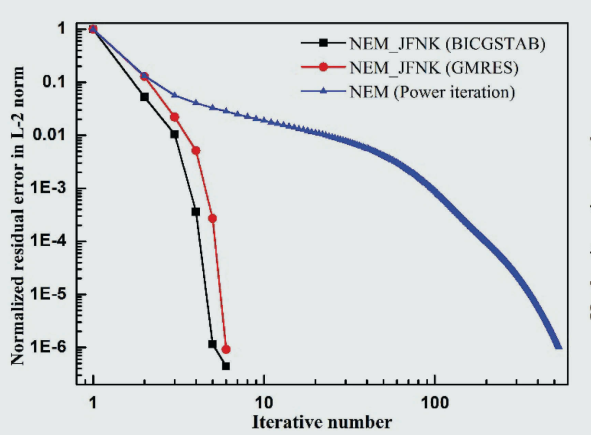
\includegraphics{./figs/iaea3d_convergence.png}
  \end{figure}
\end{frame}

\begin{frame}{\glsentrylong{ws}}
  \begin{itemize}
    \item \gls{ws} can reduce \gls{pi} method runtime by a factor of three or
      more.
    \item \citeauthor{qe2paper} do not compare the \gls{jfnk} method to a
      \gls{pi} method with the \gls{ws}.
    \item \gls{ws} could invalidate some of the results.
    \item \gls{jfnk} may still be preferable to \gls{pi}+\gls{ws} \cite{jfnk_wielandt}.
    \item \gls{ws} would also be useful for a \gls{pi} preconditioner.
  \end{itemize}
\end{frame}

\section{Conclusions and Implications}
\label{sec:conclusion}

  % seems useful in this application
  In \citetitle{qe2paper}, the authors conclude that the proposed method of
  solving the \gls{nem} equations with the \gls{jfnk} method after performing 
  local elimination and using the physics based preconditioner provides improved
  convergence rate and reduced computation time compared to their presentation
  of the \gls{pi} method. It is difficult to argue with these results as
  presented. However, \sref{sec:critique} has shown that it is the data omitted
  from the results presented that merits consideration. Otherwise, it is
  difficult to extend the results of \citeauthor{qe2paper} to general solution
  methods for the \gls{nem} equations.

  The first step for better interpreting the results presented is to compare the
  \gls{jfnk} method to a \gls{pi} method using the \gls{ws} as in the work by
  \citeauthor{jfnk_wielandt}. It would also be useful to investigate
  preconditioning with a few \glspl{pi} as this has been demonstrated to be the
  preferable preconditioning by others \cite{gill_azmy,jfnk_wielandt}. Finally,
  the \gls{nem} should be implemented in the $\dtilde$ formulation to improve
  computational efficiency and allow for compatibility with existing
  production-quality computer programs \cite{palmtagThesis,smith_nonlinear}.

  In their concluding remarks, \citeauthor{qe2paper} claim that their method
  will be extended to ``improve the computational efficiency for large-scale
  complicated multiphysics coupled problems in nuclear reactor analysis''
  \cite{qe2paper}. This may seem like a straightforward extension and it would
  serve as an important demonstration because nuclear reactor simulations are
  inherently multiphysics simulations. Typically, users do not simply want a
  solution to the \gls{nem} coefficients but are interested in other reactor
  properties such as temperatures. 

  The author's claim is extremely bold given both the lack of important results
  and other publications in the field.  Specifically, \citeauthor{caslJFNK}
  investigated this exact application of \gls{jfnk} to large-scale multiphysics
  simulations. Such an application required significant work in the formation of
  the Jacobian included constructing approximations of temperature derivatives
  of cross sections. These cross section derivatives were specific to a
  particular type of reactor (\glspl{pwr}) but \citeauthor{qe2paper} attempt to
  simulate both \glspl{pwr} and pebble bed reactor designs. Succinctly, in
  full reactor multiphysics simulations, the authors determined that without the
  calculation of cross section derivatives, the \gls{jfnk} method was
  unacceptable as it required an extreme amount of cross section processing
  time.

  The results of \citeauthor{caslJFNK} are not the end of the narrative. 
  Applying the \gls{jfnk} method to the \gls{nem} equations may be useful for
  certain nuclear reactor multiphysics simulations. However, insufficient data 
  is provided by \citeauthor{qe2paper} to make such a conclusion. Additional
  attention must be paid in the application of the \gls{jfnk} method to the
  \gls{nem} equations to determine if such an implementation would provide
  a benefit compared to existing methods.


\begin{frame}{Thank You!}
  Thank you all for coming this morning!
\end{frame}

\begin{frame}[allowframebreaks]{References}
  \nocite{*}
  \printbibliography[heading=none]
\end{frame}

\begin{frame}[allowframebreaks]{Acronyms}
  \glsaddall
  % this width could potentially allow text to flow off the page... 
  % but just don't do that...
  \setlength{\glsdescwidth}{0.8\textwidth}
  \setglossarystyle{long}
  \renewcommand{\glsnamefont}[1]{\textbf{#1}}
  \renewcommand{\glsgroupskip}{}
  \printglossary[type=\acronymtype,nonumberlist]
\end{frame}

\end{document}
